\chapter{Extended plots}
\label{appendix:a}

\begin{figure}
\centering
    \textsc{\MakeLowercase{\ws{} scenario}}\\
    \medskip
\begin{subfigure}{\linewidth}
  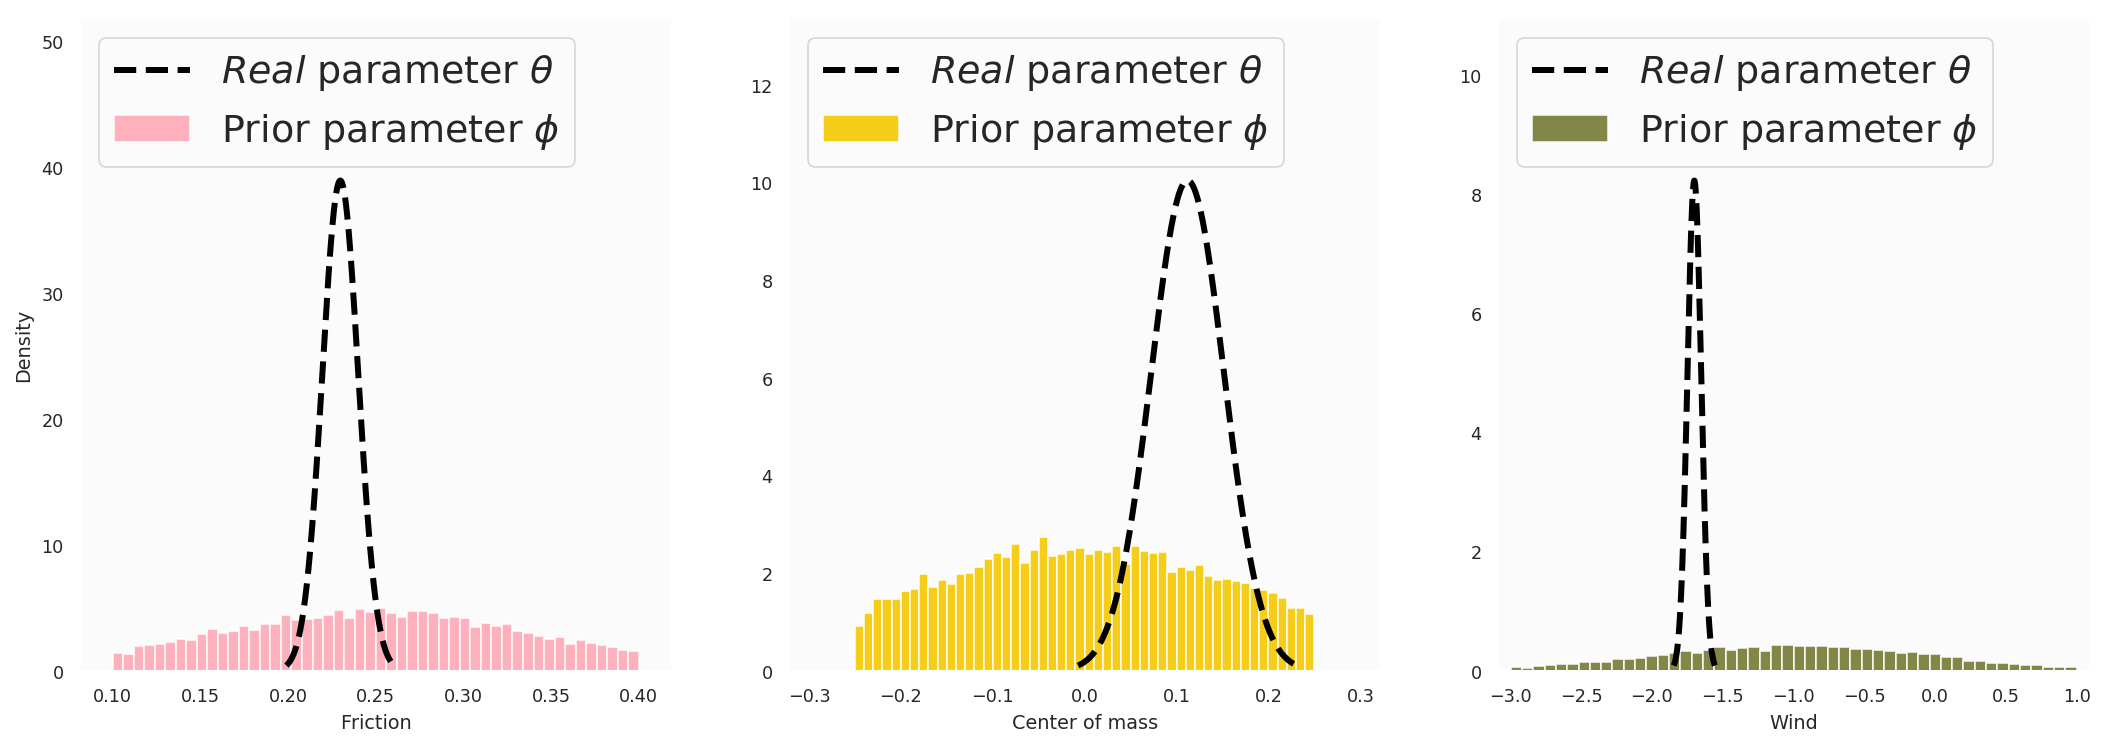
\includegraphics[width=1.0\linewidth]{img/windyslope/latent-representation/iter0_style_phi}
  \caption{Prior estimates}
\end{subfigure}
\begin{subfigure}{\linewidth}
  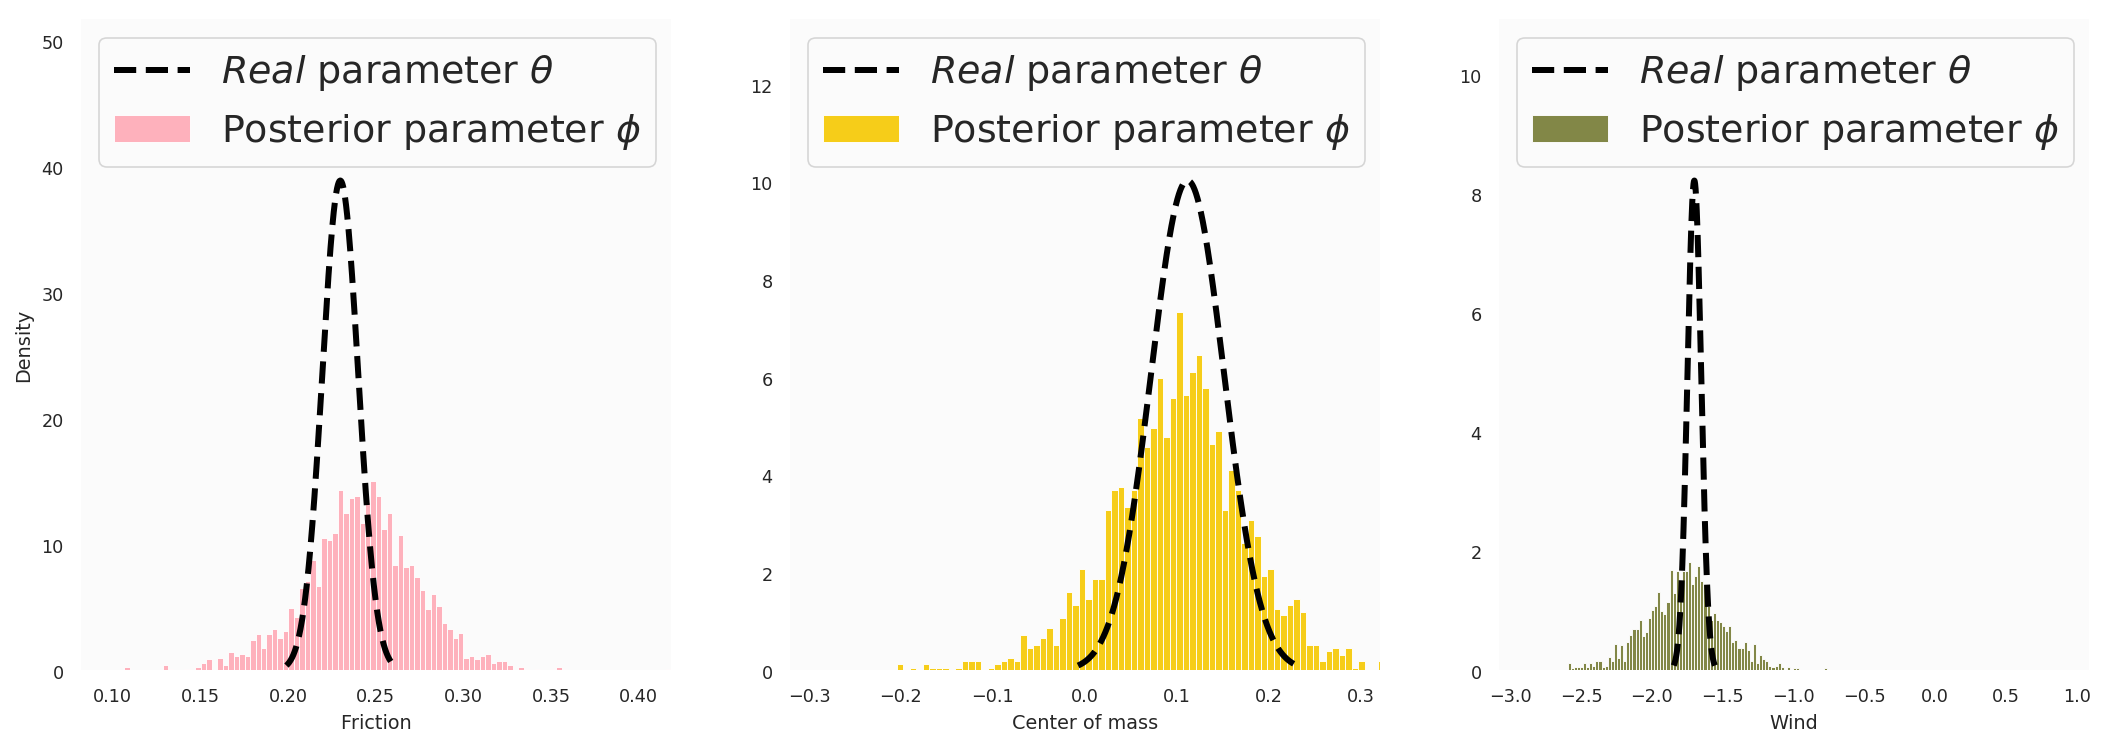
\includegraphics[width=1.0\linewidth]{img/windyslope/latent-representation/latent_encodings_iter2_8_style}
  \caption{1st iteration}
\end{subfigure}
\begin{subfigure}{\textwidth}
  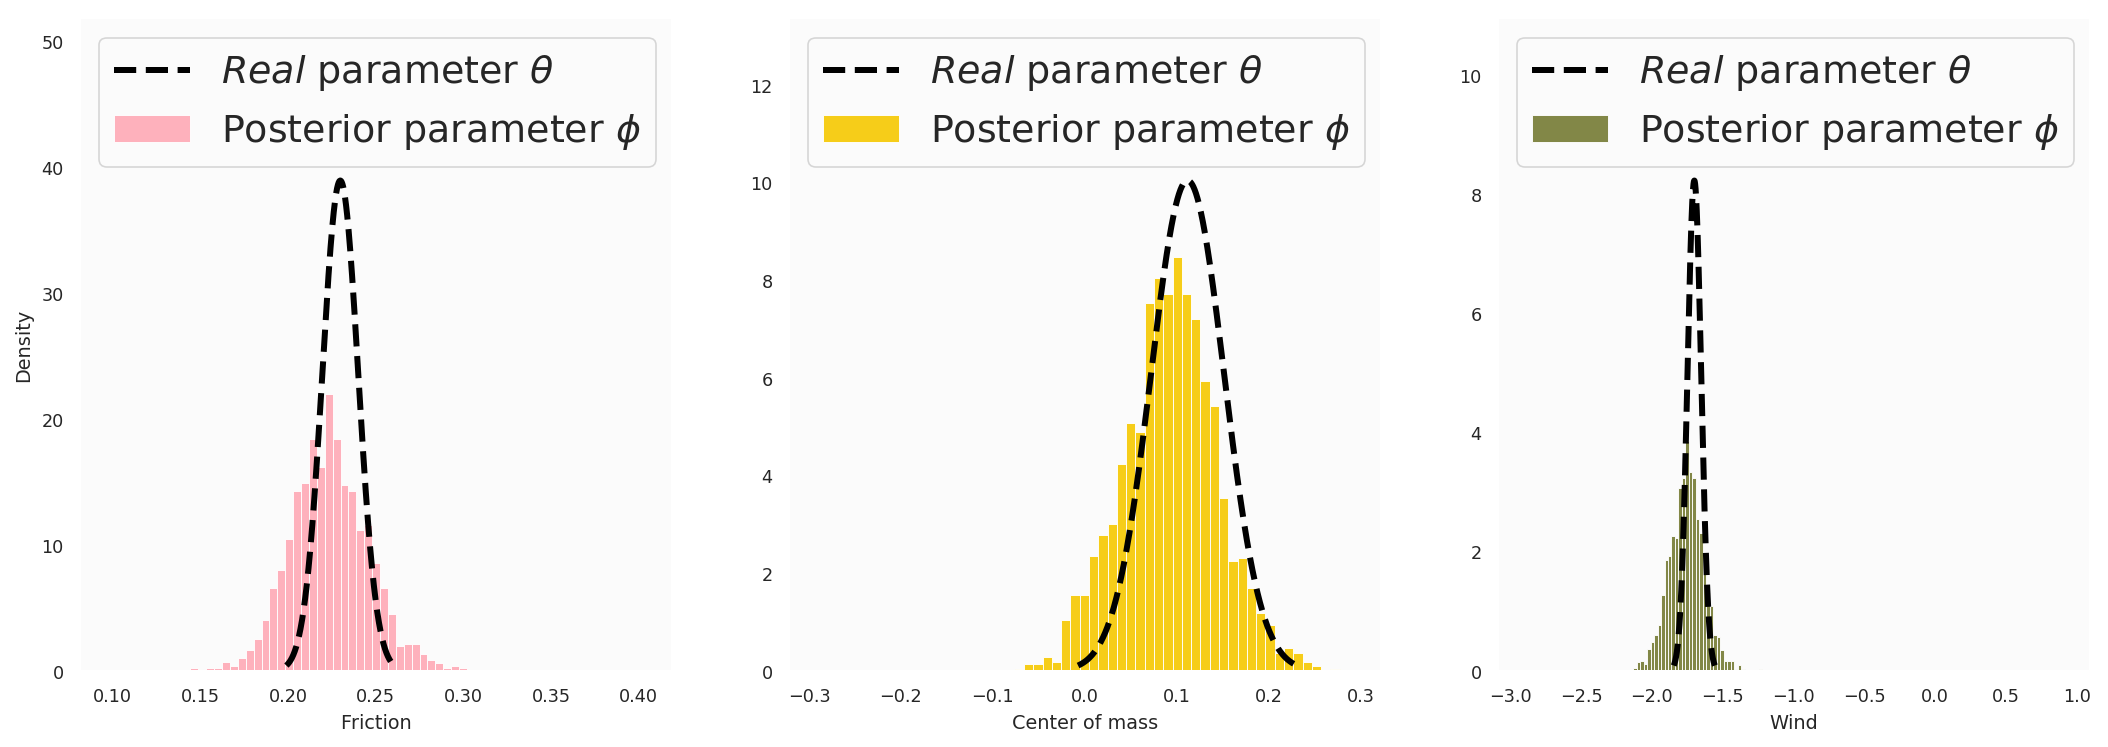
\includegraphics[width=1.0\linewidth]{img/windyslope/latent-representation/iter3_8_style2}
  \caption{2nd iteration}
\end{subfigure}
\begin{subfigure}{\textwidth}
  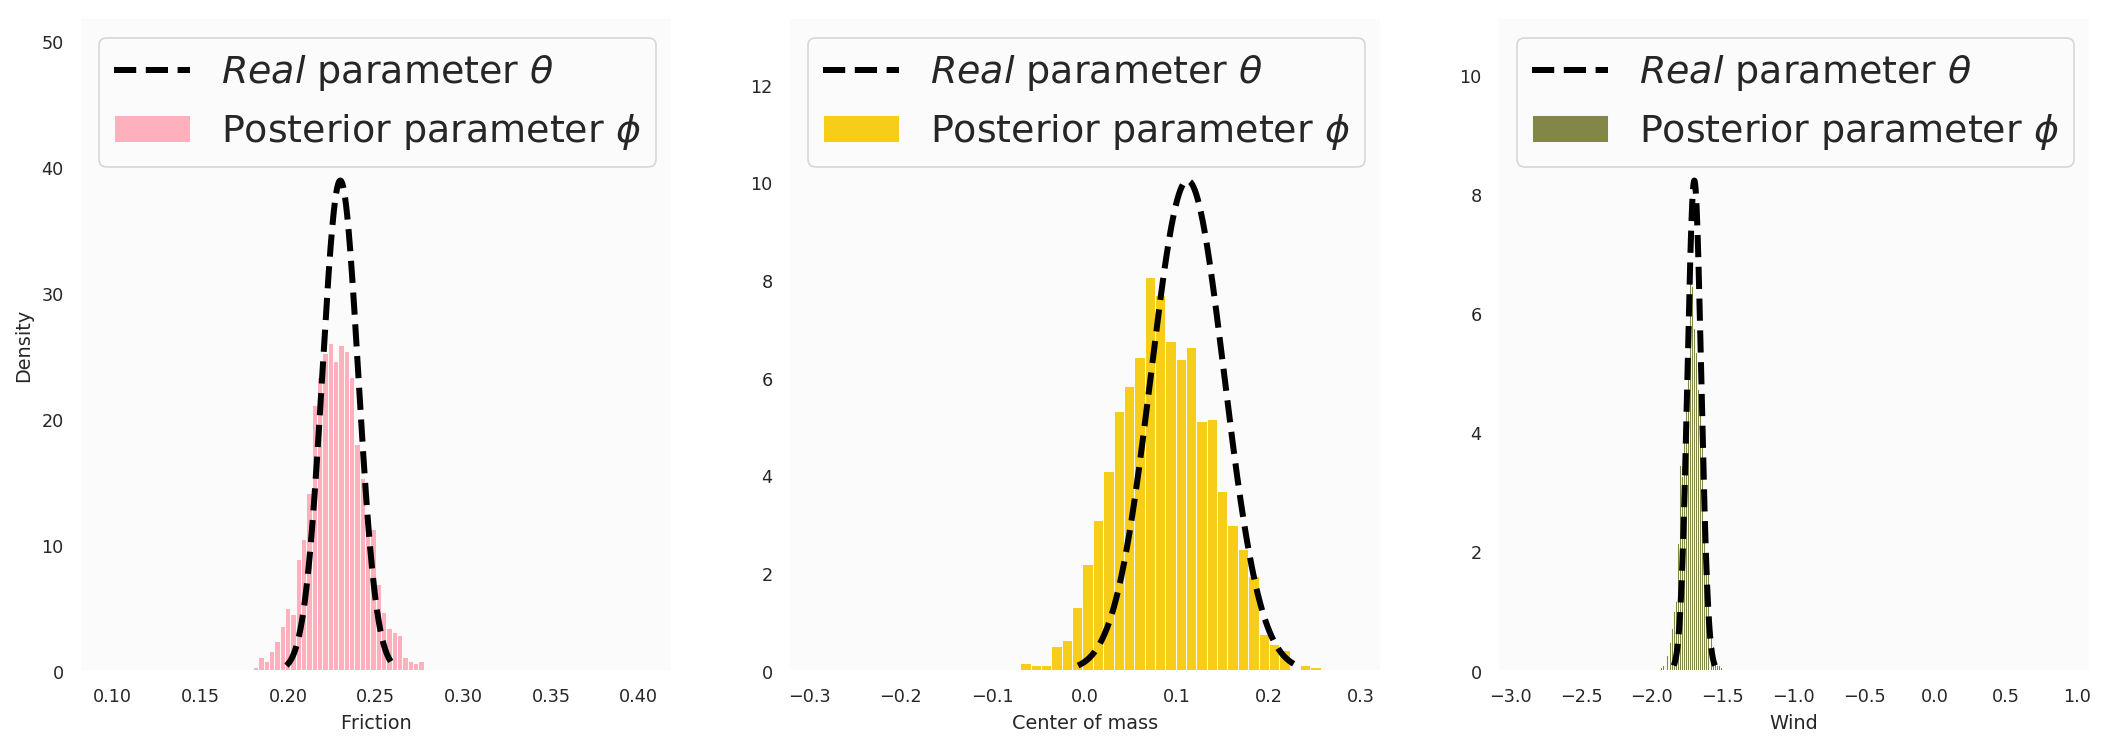
\includegraphics[width=1.0\linewidth]{img/windyslope/latent-representation/iter4_10_style}
  \caption{3rd iteration}
\end{subfigure}
\caption{Plots show the learned parameters $\vph_{\mu, \sigma}$ of the posterior given \emph{real} samples $\vec{\xi}^{real}$ as normalized histograms after subsequent steps of \dettostoc{}.
From left-to-right, the latent space codings show tangential friction, center of mass and wind. %The prior parameters $\vpsi$ for each iteration of \dettostoc{} are included for clarity in a lighter color, along with the true distribution $\theta_{\mu, \sigma}$ in black dashes.}
The \emph{real} distribution of the parameters $\theta_{\mu, \sigma}$ in drawn with black dashes.}
\label{fig:windyslope_latent_space_full}
\end{figure}

\begin{figure}
    \centering
    \textsc{\MakeLowercase{\ws{} scenario}}\\
    \medskip
    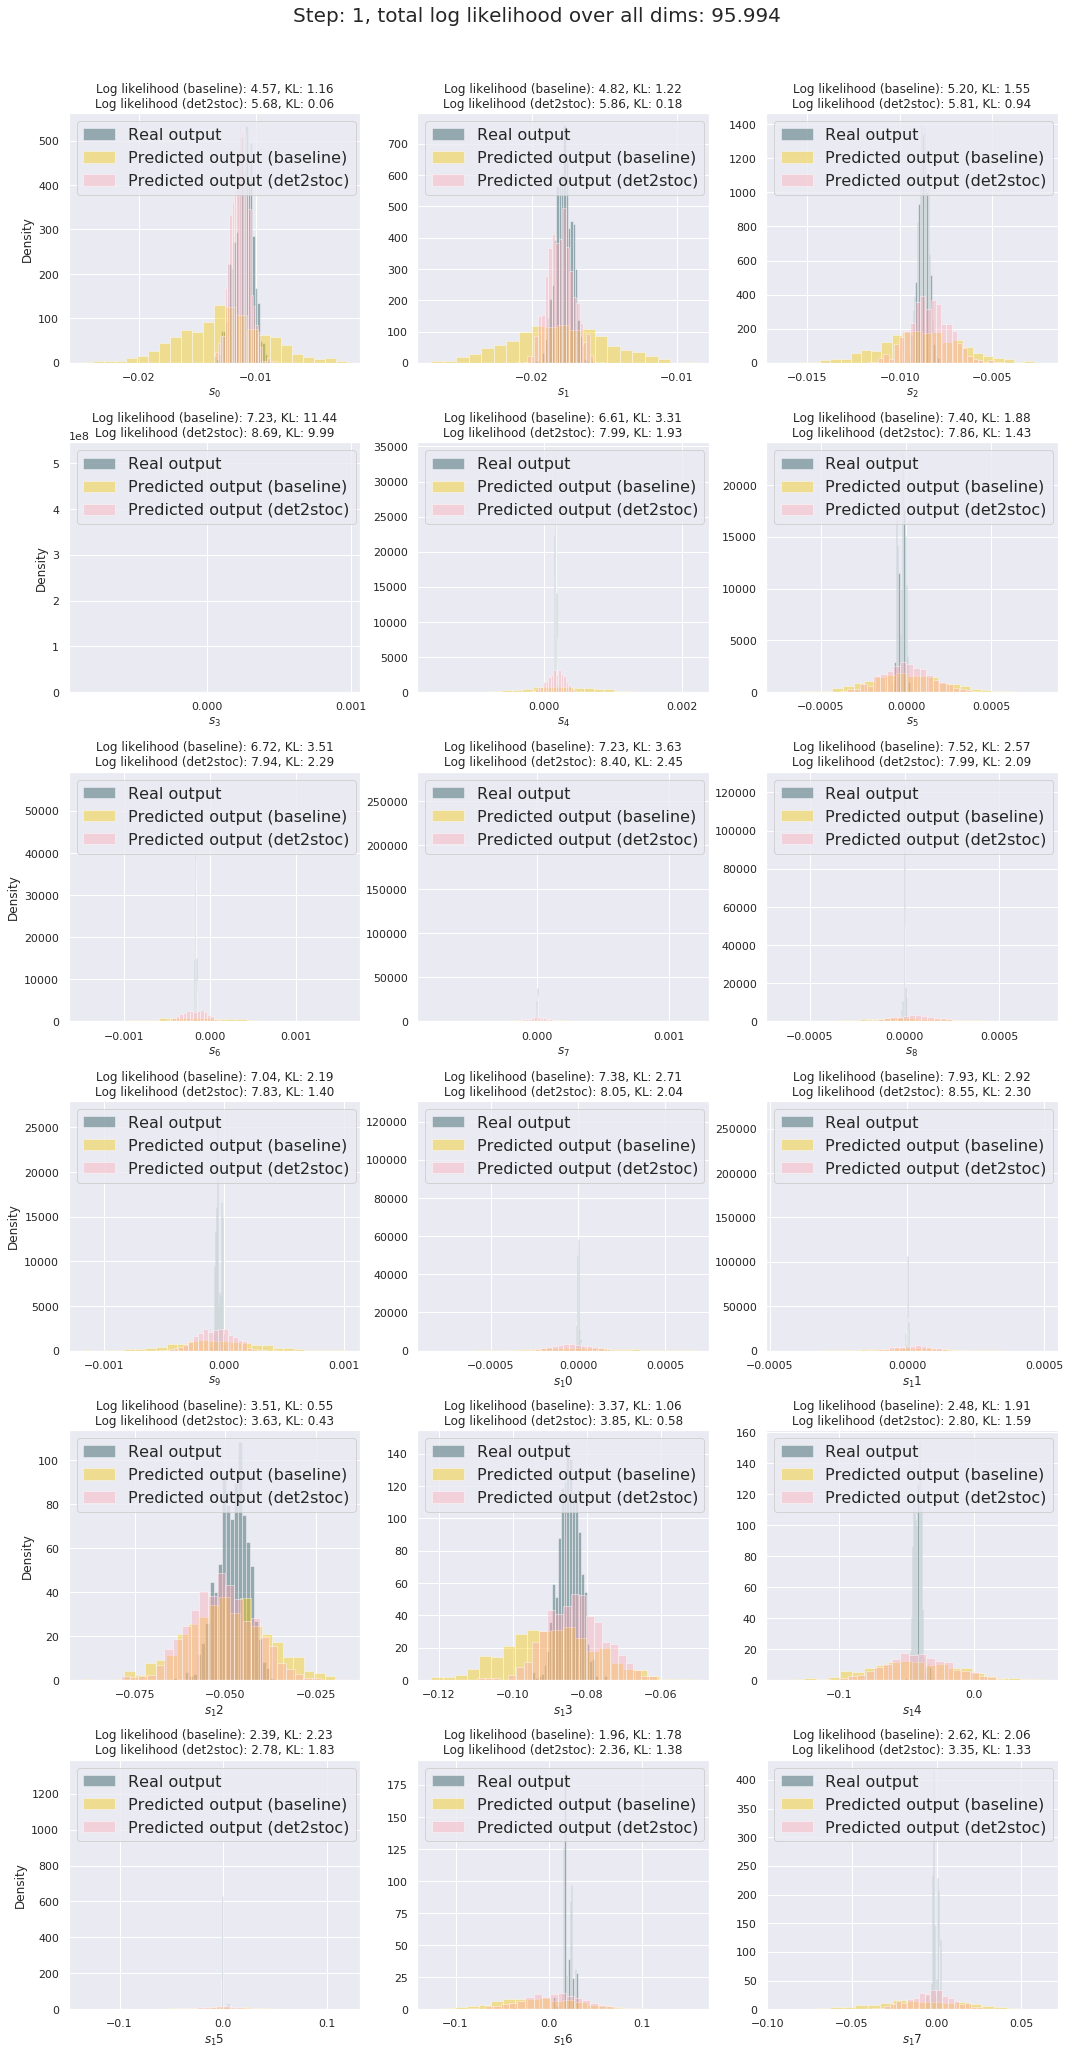
\includegraphics[width=.8\textwidth,trim=0 0 0 70,clip]{img/windyslope/output/output_distribution_step1_delta_all}
    \caption{Output predictions $\ptheta \protect\given*{\vns}{\vs}$ for a randomly sampled state at $t=1$ for iteration 3 of \dettostoc{}.}
    \label{fig:output_distribution_step1_dettostoc}
\end{figure}%

\begin{figure}
    \centering
    \textsc{\MakeLowercase{\ws{} scenario}}\\
    \medskip
    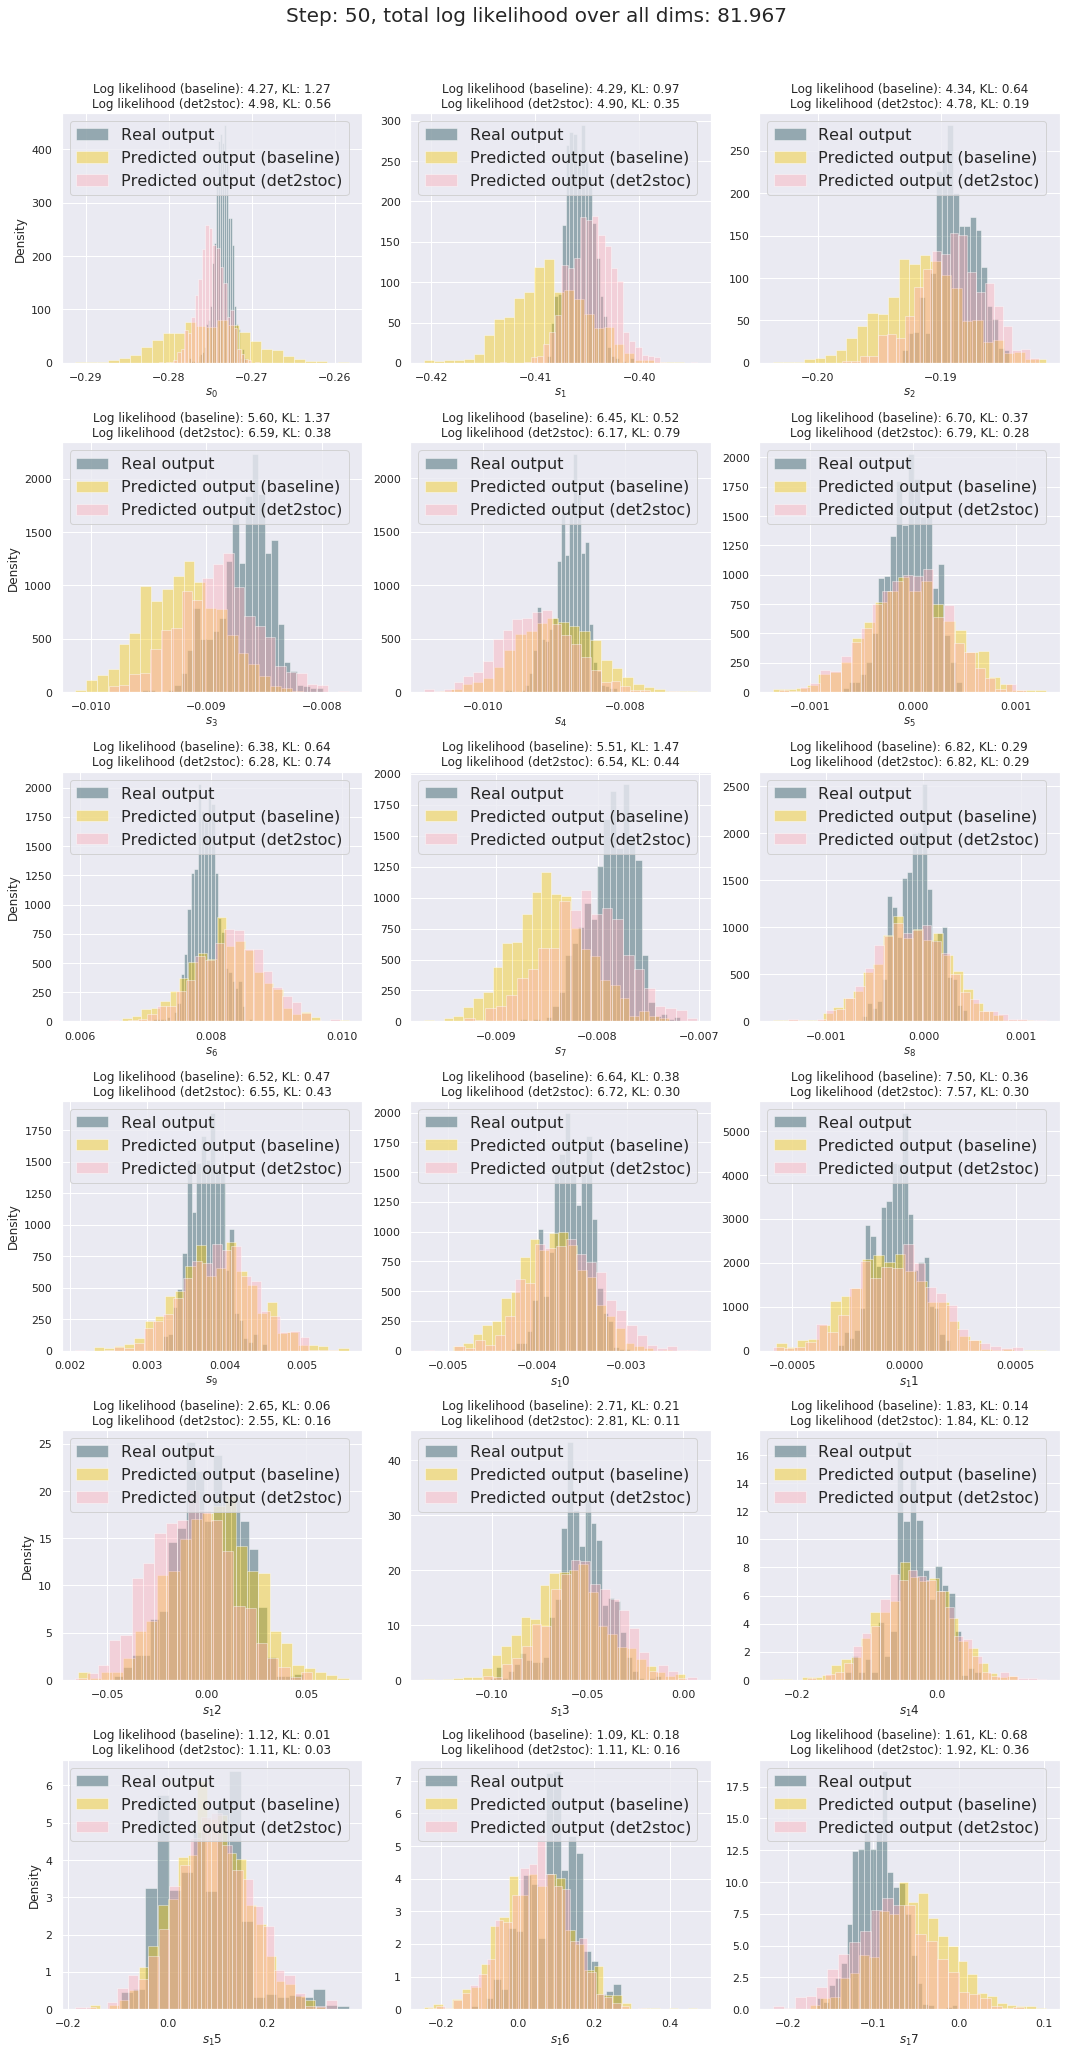
\includegraphics[width=0.8\textwidth,trim=0 0 0 70,clip]{img/windyslope/output/output_distribution_step50_delta_all}
    \caption{Output predictions $\ptheta \protect\given*{\vns}{\vs}$ for a randomly sampled state at $t=50$ for iteration 3 of \dettostoc{}.}
    \label{fig:output_distribution_step50_dettostoc}
\end{figure}

\begin{figure}
    \centering
    \textsc{\MakeLowercase{\ws{} scenario}}\\
    \medskip
    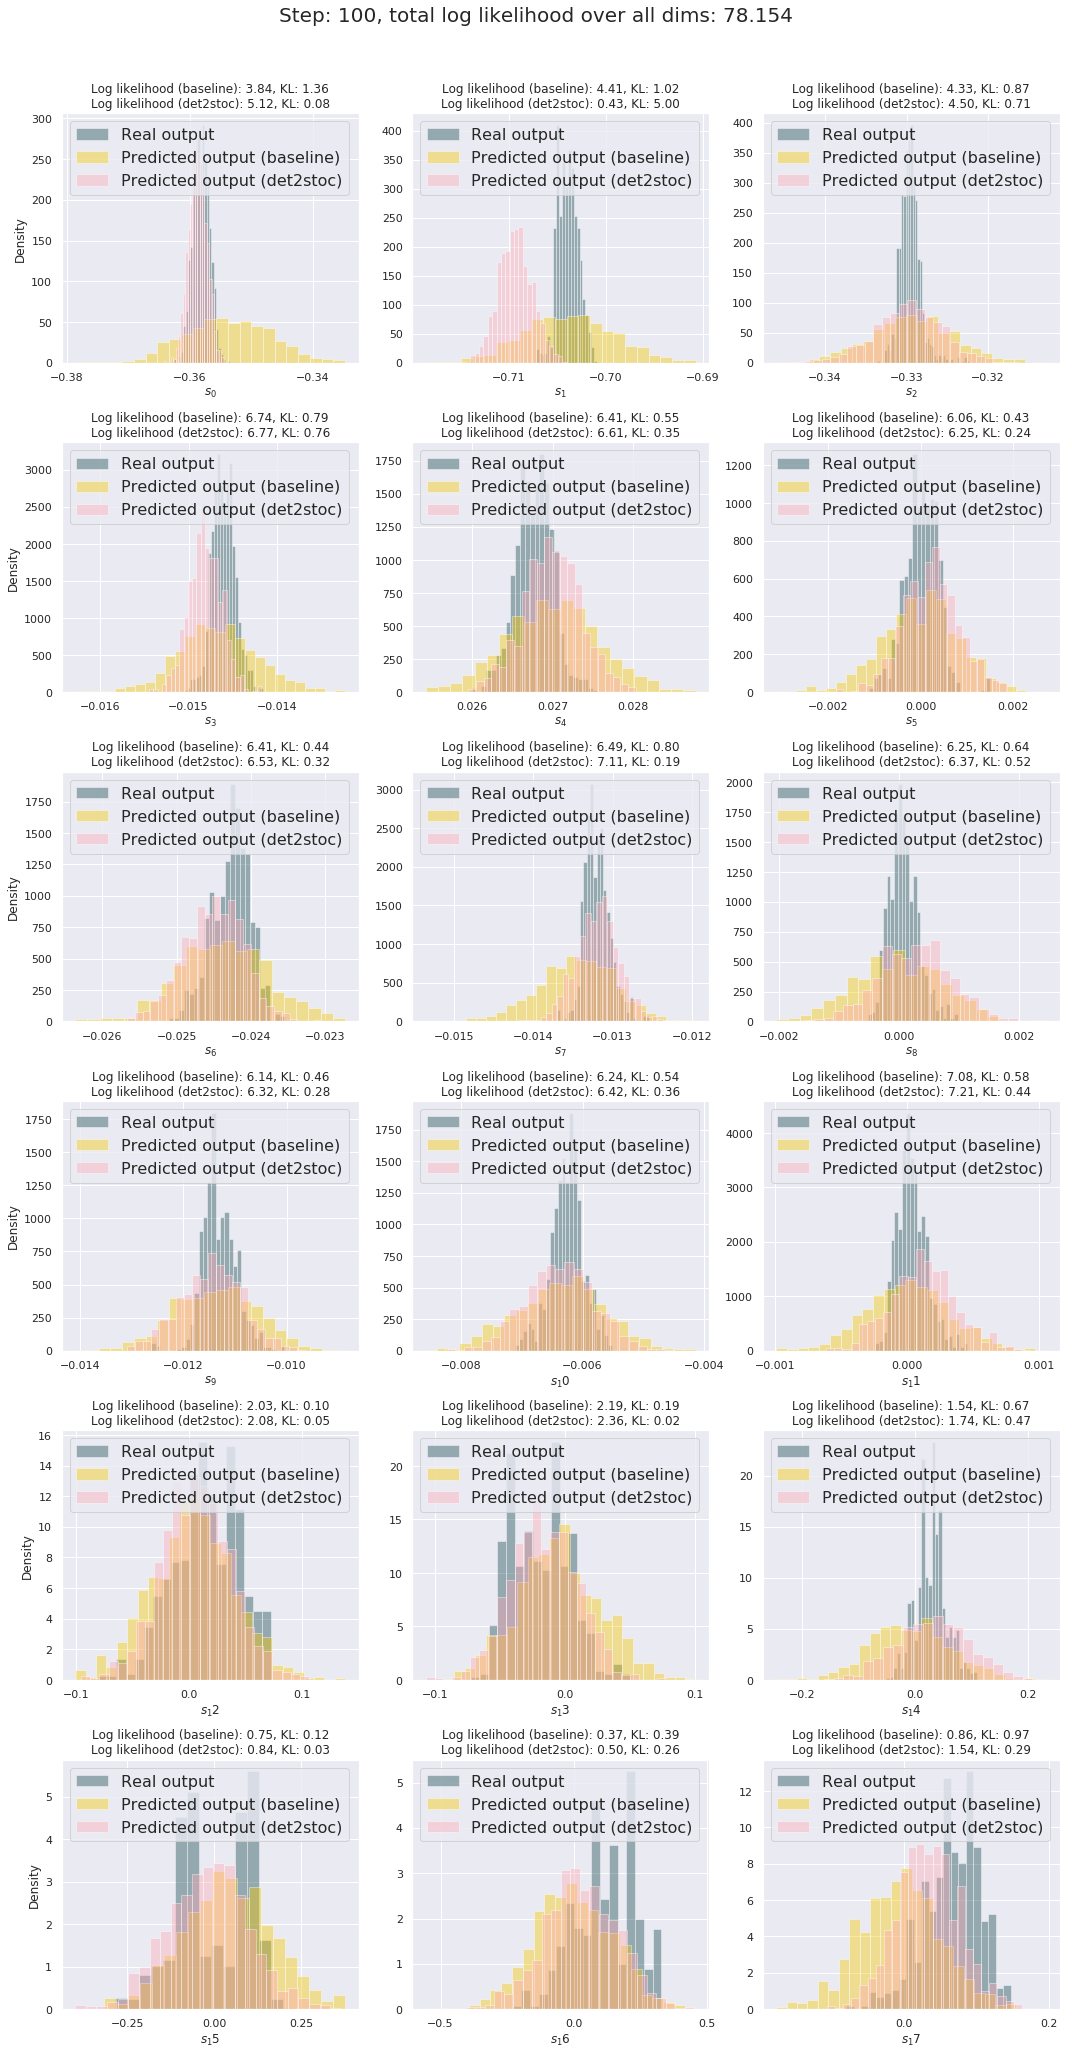
\includegraphics[width=0.8\textwidth,trim=0 0 0 70,clip]{img/windyslope/output/output_distribution_step100_delta_all}
    \caption{Output predictions $\ptheta \protect\given*{\vns}{\vs}$ for a randomly sampled state at $t=100$ for iteration 3 of \dettostoc{}.}
    \label{fig:output_distribution_step100_dettostoc}
\end{figure}


\begin{figure}
\centering
\textsc{\MakeLowercase{\yp{} scenario}}\\
\medskip
\begin{subfigure}{0.45\textwidth}
  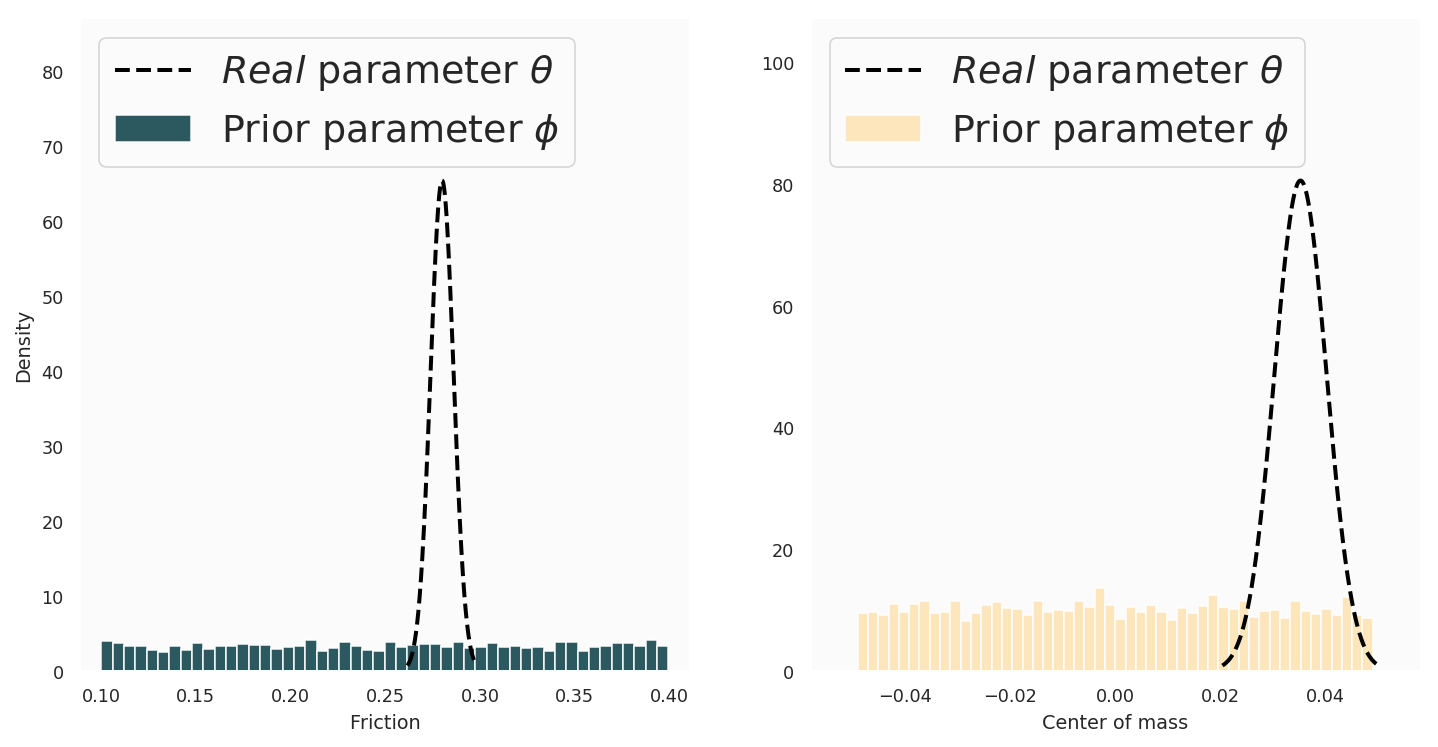
\includegraphics[width=\textwidth]{img/yumi/latent-representation/latent_encodings_iter0_style}
  \caption{Initial estimates}
\end{subfigure}
\begin{subfigure}{0.45\textwidth}
  \centering
  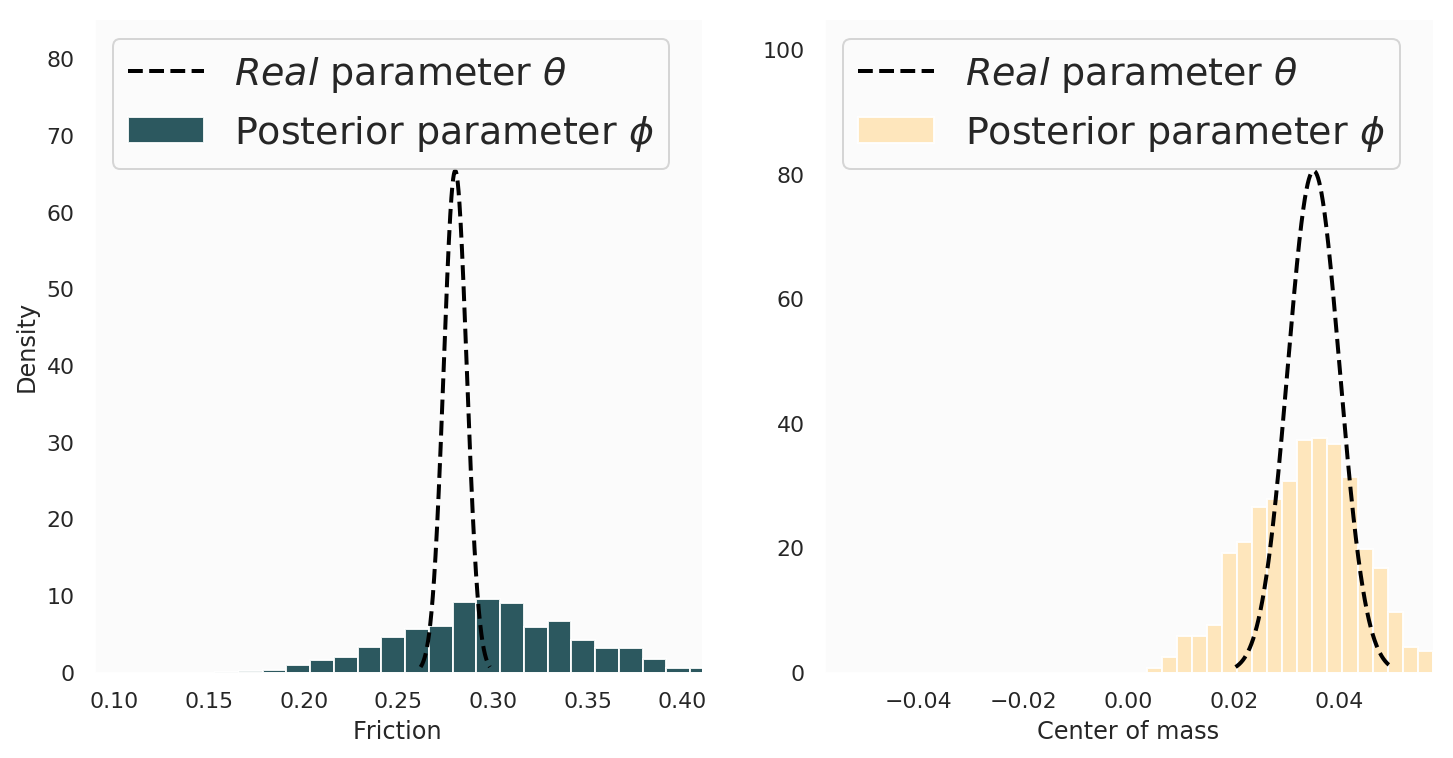
\includegraphics[width=\linewidth]{img/yumi/latent-representation/latent_encodings_iter1_style}
  \caption{1st iteration}
\end{subfigure}
\begin{subfigure}{0.45\textwidth}
  \centering
  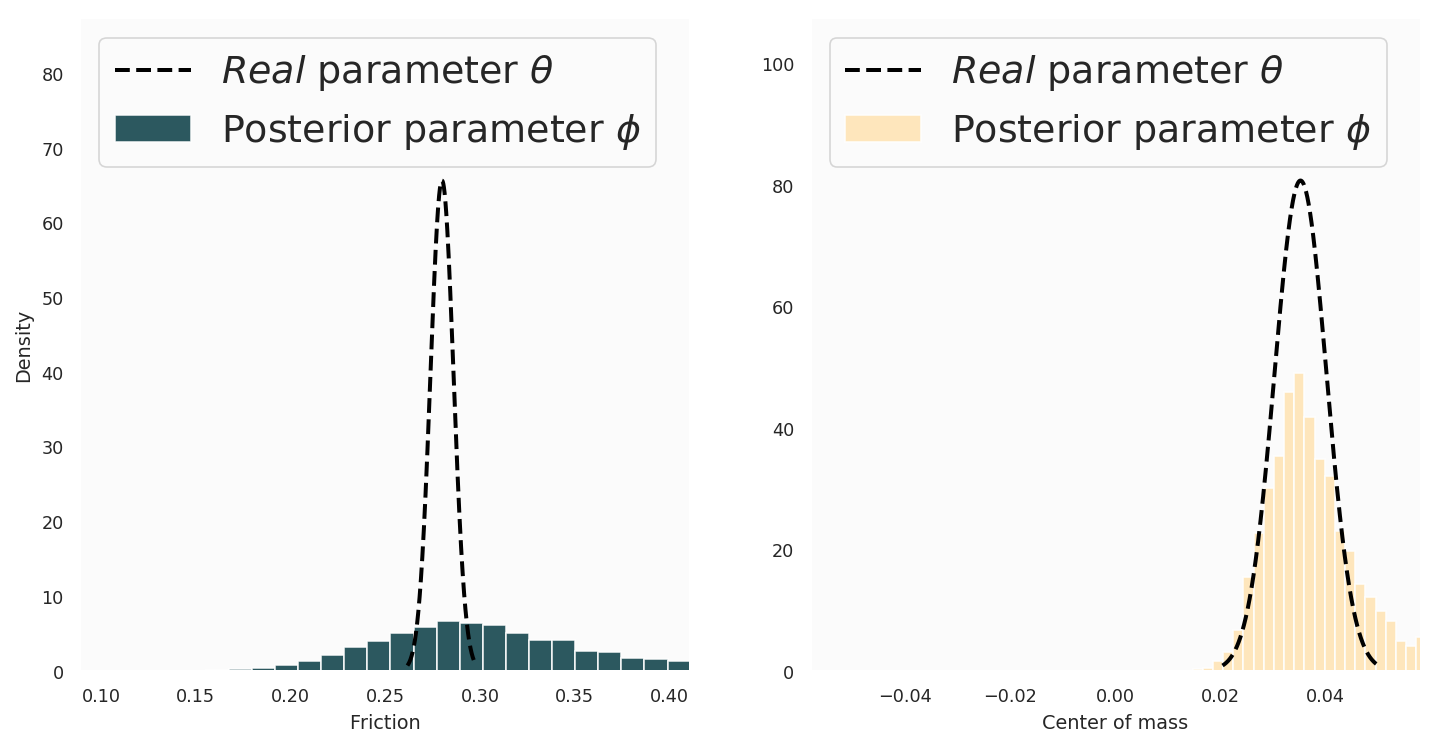
\includegraphics[width=\linewidth]{img/yumi/latent-representation/latent_encodings_iter3_10_style_3.png}
  \caption{2nd iteration}
\end{subfigure}
\begin{subfigure}{0.45\textwidth}
  \centering
  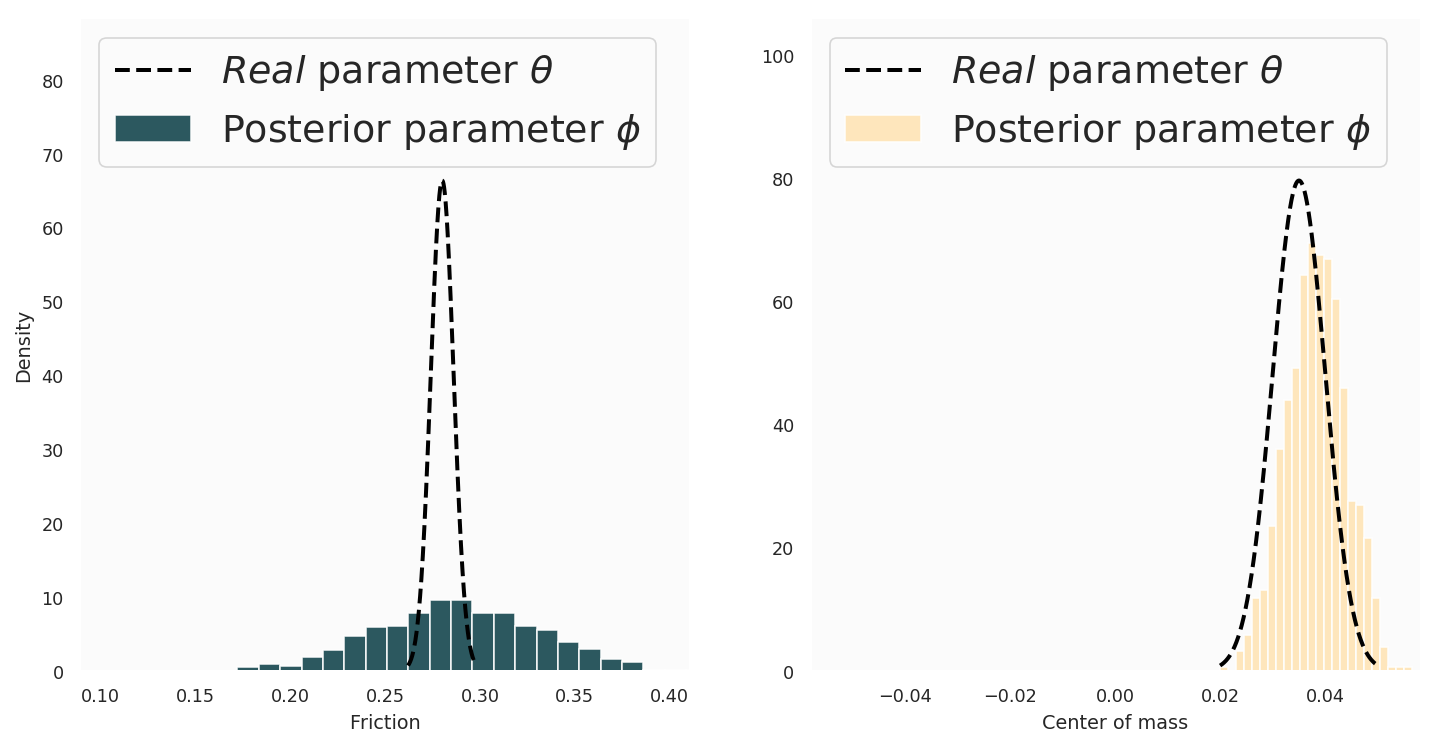
\includegraphics[width=\linewidth]{img/yumi/latent-representation/latent_encodings_iter4.png}
  \caption{3rd iteration}
\end{subfigure}
\caption{Plots show the learned parameters $\vph_{\mu, \sigma}$ of the posterior given \emph{real} samples $\trajreal$ in the \yp{} scenario for four iterations of \dettostoc{}.
The parameters correspond to tangential friction $\pfriction$ (left) and center of mass $\pcom$ (right). The true distributions $\vth_{\mu, \sigma}$ are outlined in black dashes. In this scenario, \dettostoc{} struggles to match $\pfriction{}$ with the true distribution $\theta_\textsc{friction}$. This is likely due to the fact that the learned policy pushes the box in small increments, and small changes in friction do not cause any noticeable difference. The posterior for all iterations can be found in the appendix.}
\label{fig:yumi_latent_space_full}
\end{figure}